\documentclass[12pt]{article}
\usepackage[utf8]{inputenc}
\usepackage[paper=letterpaper,margin=2cm]{geometry}
\usepackage{amsmath, array}
\usepackage{amssymb}
\usepackage{amsfonts}
% \usepackage[margin=2.5cm]{geometry}
\usepackage{enumitem}
\usepackage{titling}
% \usepackage{graphicx}
\usepackage[spanish]{babel}
\decimalpoint
\usepackage[colorlinks=true]{hyperref}
\usepackage{listingsutf8}
\usepackage[pdftex]{graphicx}
% \usepackage[export]{adjustbox}
\usepackage{caption}
\usepackage{subcaption}
\usepackage{fancyhdr}
\usepackage{multirow}
\usepackage{biblatex}
\usepackage{physics}
\usepackage{siunitx}
\usepackage[table,xcdraw]{xcolor}
\addbibresource{ref.bib}
\usepackage{tocloft}
\hypersetup{linkcolor=blue}
\newcommand{\m}{\text{m}}
\newcommand{\mpers}{\unit[per-mode = symbol]{\metre\per\second}}
\pagestyle{fancy}
\fancyhf{}

\title{Plantilla prácticas}
\author{Rodrigo Rafael Castillo Chong}
\date{\today}
\begin{document}
	
	\thispagestyle{empty}
	
	\begin{figure}[ht]
		\minipage{0.7\textwidth}
		
\includegraphics[width=4cm]{images/usaclogo.png}
		\label{EscudoUSAC}
		\endminipage
		\minipage{0.32\textwidth}
		
\includegraphics[height = 4cm ,width=4cm]{images/logoecfmplain.png}
		\label{EscudoECFM}
		\endminipage
	\end{figure}
	
	\begin{center}
		\vspace{0.8cm}
		\LARGE
		UNIVERSIDAD DE SAN CARLOS DE GUATEMALA
		
		\vspace{0.8cm}
		\LARGE
		ESCUELA DE CIENCIAS FÍSICAS Y MATEMÁTICAS
		
		\vspace{1.7cm}	
		\Large
		\textbf{Informe final de prácticas}
		
		\vspace{1.7cm}
		\Large
		\textbf{Evaluación de distintos métodos numéricos para resolver ecuaciones particulares de la mecánica de fluidos}
		
		
		\vspace{1.3cm}
		\normalsize	
		POR \\
		\vspace{.3cm}
		\large
		\textbf{Rodrigo Rafael Castillo Chong \\ 201804566}
		
		\vspace{1.3cm}
		\normalsize	
		ASESORADO POR \\
		\vspace{.3cm}
		\large
		\textbf{Enrique Pazos, Ph.D.}
		
		
		
		\vspace{1.3cm}
		\today
	\end{center}
	
	\newpage
	\tableofcontents
	\clearpage
	
	\section{Método de diferencias finitas}
	El \textbf{método de diferencias finitas} o \textbf{método DF} es un método numérico que sirve para resolver ecuaciones diferenciales. El método consiste en discretizar el dominio de la ecuación en un conjunto finito de puntos llamado \textbf{grilla}; donde cada punto debe estar a la misma distancia de cada uno de sus vecinos. Posteriormente se deben aproximar las derivadas de la función con ecuaciones de diferencias utilizando series de potencias, para poder resolver la ecuación diferencial algebraica e iterativamente \cite[1]{devries2011first}
	
	Un ejemplo de discretización que se usa al aplicar el método DF es el siguiente: la segunda derivada parcial respecto a $x$ de una función $u = u(x,t)$ valuada en $(x,t)$ se puede aproximar expandiendo la función en dos series de Taylor centradas en dos diferentes valores sobre el eje $x$ que corresponden a los dos puntos vecinos a $x$, separándose de este punto por una distancia $\Delta x$; también llamada \textbf{tamaño de paso} en $x$. 
	
	Para obtener la aproximación de la segunda derivada de $u$ respecto a $x$ usamos las expansiones en series de Taylor:
	\[u(x + \Delta x,t) \approx u(x,t) + \Delta x\pdv{u}{x}+ \frac{(\Delta x)^{2}}{2}\pdv{^{2}u}{x^2} \]
	\[u(x - \Delta x,t) \approx u(x,t) - \Delta x\pdv{u}{x}+\frac{(\Delta x)^{2}}{2}\pdv{^{2}u}{x^2} \]	
	Sumando ambas aproximaciones se obtiene:
	\[(\Delta x)^2 \pdv{^{2}u}{x^2}\approx u(x + \Delta x,t) + u(x - \Delta x,t) - 2 u(x,t)\]
	\[\pdv{^{2}u}{x^2}\approx \frac{u(x + \Delta x,t) + u(x - \Delta x,t) - 2 u(x,t)}{(\Delta x)^2}\]
	Por tanto, podemos aproximar una derivada de segundo orden en términos de valores conocidos, puesto que $u(x + \Delta x,t)$ y $u(x - \Delta x,t)$ corresponden a valores que toma la función en un dominio discretizado, en donde la distancia entre los puntos de la grilla es siempre $\Delta x$. Se puede escribir la función valuada en forma discreta:
	\[u_{i} := u(x,t)\]
	\[u_{i+1} := u(x + \Delta x,t)\]
	\[u_{i-1} := u(x - \Delta x,t)\]
	Se puede visualizar la discretización en la figura \ref{fig:discretizacion}.
	
	\begin{figure}[ht]
		\centering
		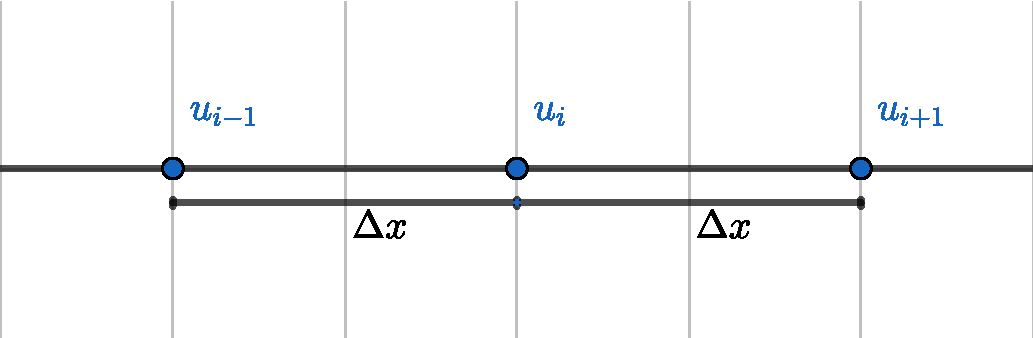
\includegraphics[scale=0.8]{images/grilla.pdf}
		\caption{Discretización del dominio espacial}
		\label{fig:discretizacion}
	\end{figure}
	
	
	En general, el dominio temporal de la función también se discretiza, tomando intervalos de tiempo consecutivos separados por un intervalo de tiempo $\Delta t$ o también llamado tamaño de paso en $t$. 
	
	Para aproximar la primera derivada parcial en $t$ de $u$ se expande la función en una serie de Taylor centrada en $\Delta t$ y el término donde la función está valuada en el instante temporal más futuro se renombra como $u_{\text{nueva}}$.
	
	\[u(x,t+\Delta t)\approx u(x,t) + \Delta t \pdv{u}{t}\]
	\[\pdv{u}{t} \approx \frac{u(x,t+\Delta t) - u(x,t)}{\Delta t}\]
	\[\pdv{u}{t} \approx \frac{u_{\text{nueva,} i} - u_{i}}{\Delta t}\]
	
	Posteriormente se reemplazan las discretizaciones aproximadas en la ecuación diferencial a resolver y se itera sobre las variables dependientes de acuerdo al tamaño del dominio discretizado. 
	
	En resumen, el método DF funciona aproximando y adaptando las derivadas de primer y segundo orden a ecuaciones de diferencias que dependen de los valores que la función devuelve cuando esta se valúa en los puntos de la grilla, o bien, en instantes discretos de tiempo.\\
	
	
	A continuación se describen los problemas resueltos con el método de diferencias finitas y los resultados conseguidos con este.

	
	\subsection{Ecuación de Burgers no viscosa, en una dimensión}
	La ecuación de Burgers no viscosa en una dimensión espacial es una ecuación diferencial parcial de primer orden que expresa la evolución temporal de la cantidad $u = u(x,t)$, la cual puede ser interpretada como la componente en $x$ de la \textbf{velocidad} de un fluido o gas. La ecuación tiene la siguiente forma:
	\begin{equation}
		\pdv{u}{t}+u\pdv{u}{x}=0
		\label{eq:burgers1d}
	\end{equation}
	
	Se resolvió esta ecuación en un dominio espacial dado por $x \in [0,\text{L}]$, donde $\text{L} = 100 \unit{\meter}$, y sujeta a las siguientes condiciones iniciales:\\
	\begin{equation}
		u(0,0)=0
	\end{equation}
	\begin{equation}
		u(\text{L},0)= 0
	\end{equation}
	Estas condiciones pueden interpretarse como el modelado de un fluido sin presión ni viscosidad, o un gas, que se mueve en una dimensión cuyos extremos simulan un tope o frontera que impide que el fluido o gas en cuestión salga. %Se tomó $\text{L}=100\m$ como el largo del dominio.
	
	Como condición inicial se eligió una distribución gaussiana de velocidad. Esta se puede interpretar como un pulso centrado en el centro del dominio. Es común utilizar pulsos gaussianos como condiciones iniciales, para así visualizar su desplazamiento a lo largo de la simulación\footnote{En las ecuaciones se mantuvieron los nombres de las variables utilizadas en el código de la integración numérica de la ecuación, salvo por $\mu$ que se escribió como \texttt{mu}.}.
	\begin{equation}
		u(x,0) = A\exp(-b(x-\mu)^{2})
	\end{equation}
	\\
	Donde:
	\begin{itemize}
		\item $A=3.5\mpers$
		\item $b=0.05$
		\item $\mu=L/2=50\unit{\meter}$
	\end{itemize}
	\subsubsection*{Aplicación del método}
	Para resolver numéricamente la ecuación \ref{eq:burgers1d} utilizando el método DF, primero se debe discretizar la ecuación aproximando las derivadas parciales. Esto es:
	\begin{equation}
		\pdv{u}{x} \approx \frac{u(x+\Delta x,t)-u(x,t)}{\Delta x}
	\end{equation}
	\begin{equation}
		\pdv{u}{x} \approx \frac{u_{i+1}-u_{i}}{\Delta x}
	\end{equation}
	\begin{equation}
		\pdv{u}{t} \approx \frac{u_{\text{nueva},i}-u_{i}}{\Delta t}
	\end{equation}
	Donde $\Delta x$ y $\Delta t$ son los tamaños de paso en la dimensión espacial y temporal respectivamente\footnote{En el código, estas cantidades fueron nombradas como \texttt{dx} y \texttt{dt} respectivamente}. Sustituyendo las anteriores aproximaciones en \ref{eq:burgers1d}, obtenemos
	\begin{equation}
		\frac{u_{\text{nueva},i}-u_{i}}{\Delta t}+u_{i}\left( \frac{u_{i+1}-u_{i}}{\Delta x}\right) =0
	\end{equation}
	Luego se despeja $u_{\text{nueva},i}$
	\begin{equation}
		u_{\text{nueva,}i} = u_{i}\left[ 1 + \frac{\Delta t}{\Delta x}(u_{i}-u_{i+1}) \right]
		\label{eq:burgdiscr}
	\end{equation}
	De esta forma, el valor de la función $u$ en el i-ésimo elemento de la grilla, en un instante $t + \Delta t$, está dado por el miembro derecho de la ecuación \ref{eq:burgdiscr}, que toma valores de $u$ en un mismo instante $t$. Esta es una relación de recurrencia sobre la cual se puede iterar para construir la solución general de la ecuación.
	\clearpage
	\section{Método de volúmenes finitos}
	\section{Método de elementos finitos}
	\section{Conclusiones}
	
	\printbibliography
	
\end{document}
